\chapter{ \toolName の機能と外観}\label{cha:Function}
\toolName (Mix Visual Regression Test)は、レイアウトの不具合の発見を支援する、視覚的回帰テスト支援ツールである。
本章では、本研究で試作したツール\toolName の機能と外観について説明する。
なお、「差分箇所」、「影響箇所」、「レイアウトの副作用箇所」、「レイアウトの不具合箇所」を、以下に定義する。
\begin{itemize}
    \item 差分箇所:\\
          変更前後のWebページを比較して、
          変更前のWebページで削除された箇所と変更後のWebページで追加された箇所。
    \item 影響箇所:\\
          変更前後のWebページのHTMLコードを比較して、
          HTMLコードにおけるbody要素内の変更とstyle要素内の変更のどちらか、
          または両方の影響を受けた画面要素箇所。
    \item レイアウトの副作用箇所:\\
          変更前後のWebページでHTMLコードの変更による影響を受けた画面要素によって、
          HTMLコードを変更していない画面要素にレイアウトの変更があった箇所。
    \item レイアウトの不具合箇所:\\
          レイアウトの副作用箇所に画面要素の隠れ、見切れ、重なりがあった箇所。
\end{itemize}
% \paragraph{差分箇所}
% 変更前後のWebページを比較して、
% 変更前のWebページで削除された箇所と変更後のWebページで追加された箇所。
% \paragraph{影響箇所}
% 変更前後のWebページのHTMLコードを比較して、
% HTMLコードにおけるbody要素内の変更とstyle要素内の変更のどちらか、
% または両方の影響を受けた画面要素箇所。
% \paragraph{レイアウトの副作用箇所}
% 変更前後のWebページでHTMLコードの変更による影響を受けた画面要素によって、
% HTMLコードを変更していない画面要素にレイアウトの変更があった箇所。
% \paragraph{レイアウトの不具合箇所}
% レイアウトの副作用箇所に画面要素の隠れ、見切れ、重なりがあった箇所。

\section{\toolName の機能}
\subsection{実行コマンド}\label{subsec:MixVRT_execution}
\toolName は、Python3.9.17\cite{Python}が動作するテキスト端末上で実行する。
\toolName 実行時のコマンドライン引数によって、視覚的回帰テストを行う対象のWebページのURLを指定する。
\toolName の実行コマンドの書式は、以下である。
\begin{lstlisting}[label=list:command,frame=none,numbers=none,basicstyle={\normalsize \ttfamily \color[gray]{.15}}]
  $ make test URL="WebページのURL"
 \end{lstlisting}
{\tt URL}には、テスト対象とするWebページのURLを指定する。なお、"https://"または"http://"から始まるURLとする。
また、初回実行時のみにおいて、{\tt URL}には、視覚的回帰テストを行うための比較対象とするWebページのURLを指定する。

% \toolName の初回実行時は、比較対象となるWebページの画像とHTMLコードが存在せず視覚的回帰テストを行えないため、
% 比較対象とするWebページのURLからWebページの画像とHTMLコードの取得のみを行い、処理を終了する。
% \toolName の2回目実行時は、テスト対象とするWebページのURLからWebページの画像とHTMLコードを取得し、
% 比較対象とするWebページの画像とHTMLコードに対して視覚的回帰テストを行う。
% \toolName の3回目以降実行時は、実装の都合上、前回の視覚的回帰テストの結果に関わらず、
% 前回実行時で取得したWebページの画像とHTMLコードを比較対象とし、
% テスト対象とするWebページのURLから取得したWebページの画像とHTMLコードを用いて視覚的回帰テストを行う。
% \par
\subsection{事前準備}\label{subsec:MixVRT_preparation}
開発者は\toolName による視覚的回帰テストを行うための事前準備を行う必要がある。
事前準備は、\toolName の実行コマンド(\ref{subsec:MixVRT_execution}節を参照)を実行するだけである。
\toolName の初回実行により、視覚的回帰テストを行うための比較用画像と比較用HTMLコードを\toolName に保存する。

\subsection{入出力}\label{subsec:MixVRT_IO}
開発者は、\toolName の事前準備(\ref{subsec:MixVRT_preparation}節を参照)を行った状態で、
テスト対象とするWebページのURLを入力として\toolName の実行コマンド(\ref{subsec:MixVRT_execution}節を参照)を実行することで視覚的回帰テストを行える。
\toolName の2回目以降実行によって取得したWebページのテスト対象画像とテスト対象HTMLコードを、比較用画像と比較用HTMLコードに対して視覚的回帰テストを行うことで、
以下に示すPNG形式の画像を出力する。なお、比較用画像をWebページの変更前画像、テスト対象画像をWebページの変更後画像とする。
\begin{itemize}
    \item Webページの変更前画像と変更後画像
    \item 画像比較に基づく差分箇所を色付きの枠で囲んで強調表示した、Webページの変更前画像と変更後画像
    \item HTMLコードの変更に基づく影響箇所を色付きの枠で囲んで強調表示した、Webページの変更前画像と変更後画像
    \item レイアウトの不具合箇所を色付きの枠で強調表示した、Webページの変更前画像と変更後画像
\end{itemize}
\toolName が出力するPNG形式の画像は、Flask(\ref{sec:Flask}節を参照)を使用して構築したサーバ上で動作するローカルWebページで確認できる。
なお、\toolName の初回実行時は、テスト対象画像とテスト対象HTMLコードが存在せず視覚的回帰テストを行えないため、Webページの変更前画像のみを確認できる。

\subsection{比較用画像と比較用HTMLの更新}\label{subsec:MixVRT_evaluate}
視覚的回帰テストで問題を見つけた場合、開発者はWebページを修正し、\toolName を用いて再度テストを実行して修正が正しいかを検証する。
問題がなければ、開発者は下記の実行コマンドを実行することで、最新のテスト対象画像とテスト対象HTMLコードをそれぞれ比較用画像と比較用HTMLコードとして更新できる。
\begin{lstlisting}[label=list:command,frame=none,numbers=none,basicstyle={\normalsize \ttfamily \color[gray]{.15}}]
    $ make save
\end{lstlisting}

\section{\toolName の外観}
\toolName の外観を、図\ref{fig: Appearance}に示す。
\begin{figure}[tp]
    \begin{center}
        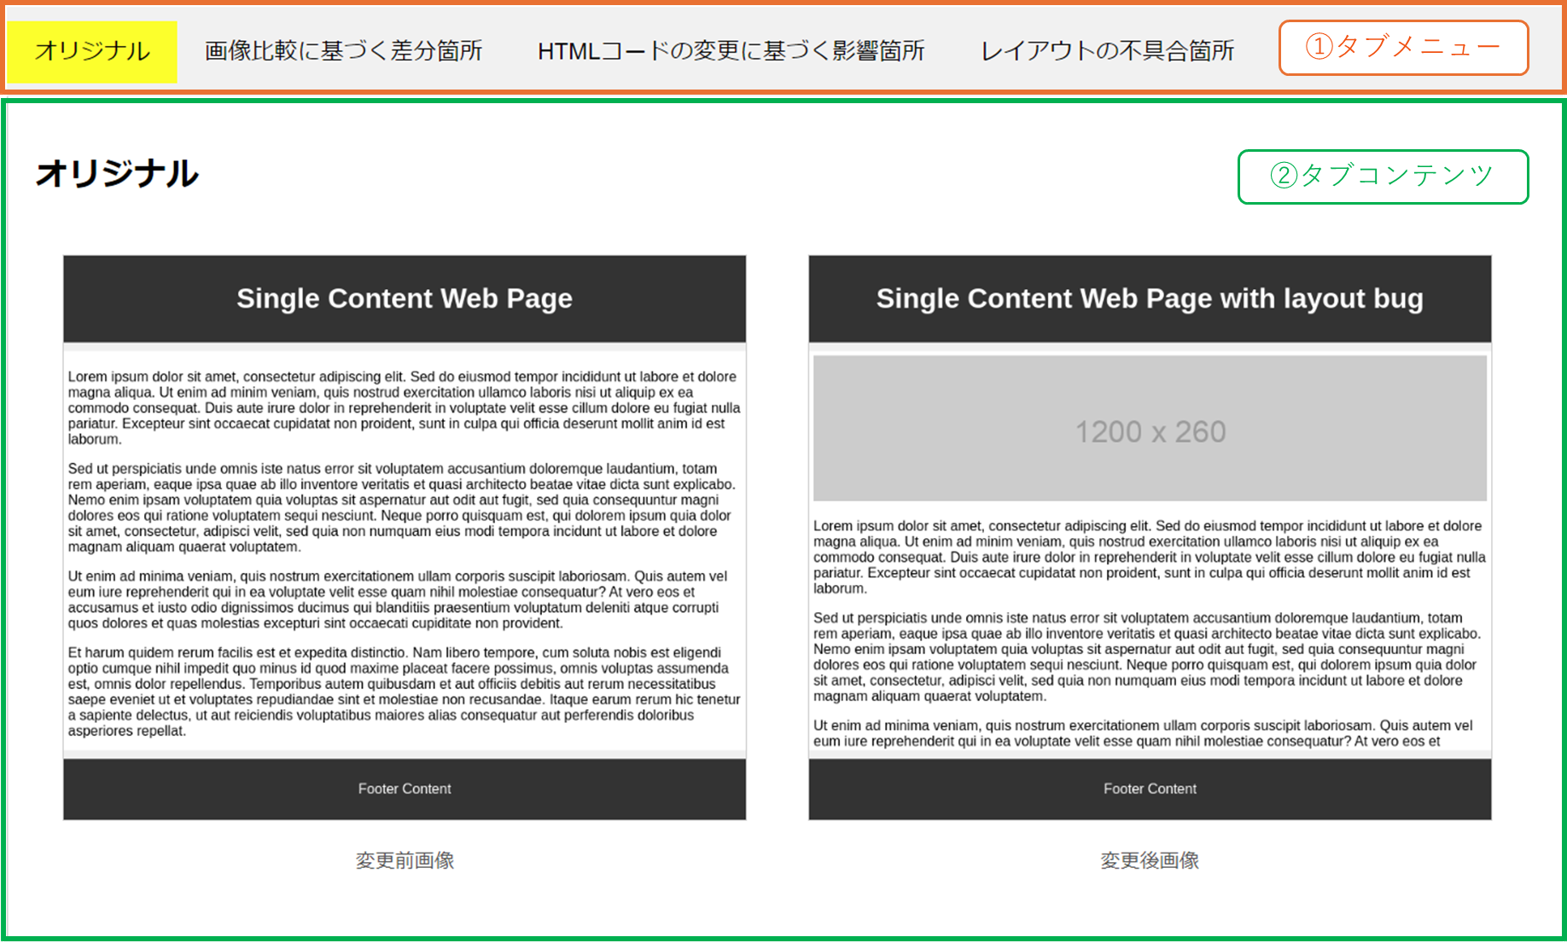
\includegraphics[width=1.0\columnwidth]{image/3_Appearance2.png}
        \caption{\toolName の外観}
        \label{fig: Appearance}
    \end{center}
\end{figure}
\toolName は、以下に示す4つのタブからなるタブメニューと各タブに対応した内容を表示するタブコンテンツからなる。
なお、以下の数字は、図\ref{fig: Appearance}の数字と対応している。
\begin{itemize}
    \item[①] タブメニュー
          \begin{itemize}
              \item オリジナル表示タブ
              \item 画像比較に基づく差分箇所表示タブ
              \item HTMLコードの変更に基づく影響箇所表示タブ
              \item レイアウトの不具合箇所表示タブ
          \end{itemize}
    \item[②] タブコンテンツ
\end{itemize}
\par
以降、各タブの外観と機能について説明する。

\subsection{オリジナル表示タブ}\label{subsec:original_tab}
オリジナル表示タブを押すと、Webページの変更前画像と変更後画像を並べて表示する。
オリジナル表示タブを押した際の\toolName の画面例を、図\ref{fig: Appearance_original_tab}に示す。
なお、\toolName に一番最初にアクセスした時やリロードした時は、デフォルトでオリジナル表示タブを選択した状態になっている。
このタブでは、Webページの変更前後の画像を目視で確認できる。
\begin{figure}[tp]
    \begin{center}
        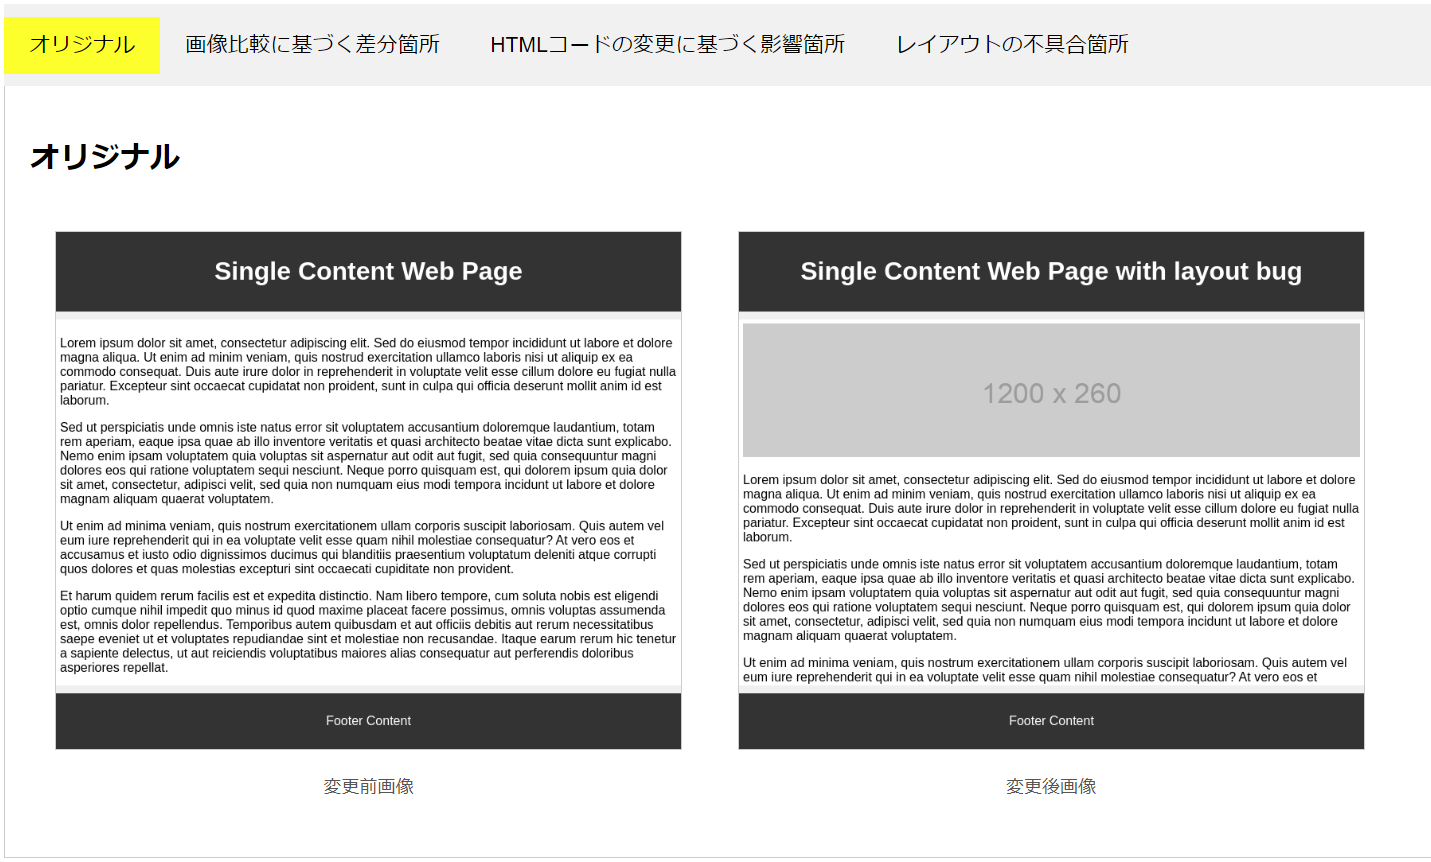
\includegraphics[width=1.0\columnwidth]{image/3_original_tab2.png}
        \caption{オリジナル表示タブを押した際の\toolName の画面例}
        \label{fig: Appearance_original_tab}
    \end{center}
\end{figure}

\subsection{画像比較に基づく差分箇所表示タブ}\label{subsec:images_tab}
画像比較に基づく差分箇所表示タブを押すと、画像比較に基づく差分箇所を色付きの枠で囲んで強調表示した、Webページの変更前画像と変更後画像を並べて表示する。
画像比較に基づく差分箇所表示タブを押した際の\toolName の画面例を、図\ref{fig: Appearance_images_tab}に示す。
削除された箇所は変更前画像上に赤枠で囲んで強調表示し、追加された箇所は変更後画像上に緑枠で囲んで強調表示する。
このタブでは、変更前後のWebページでレイアウトの変更があった箇所を目視で確認できる。
\begin{figure}[tp]
    \begin{center}
        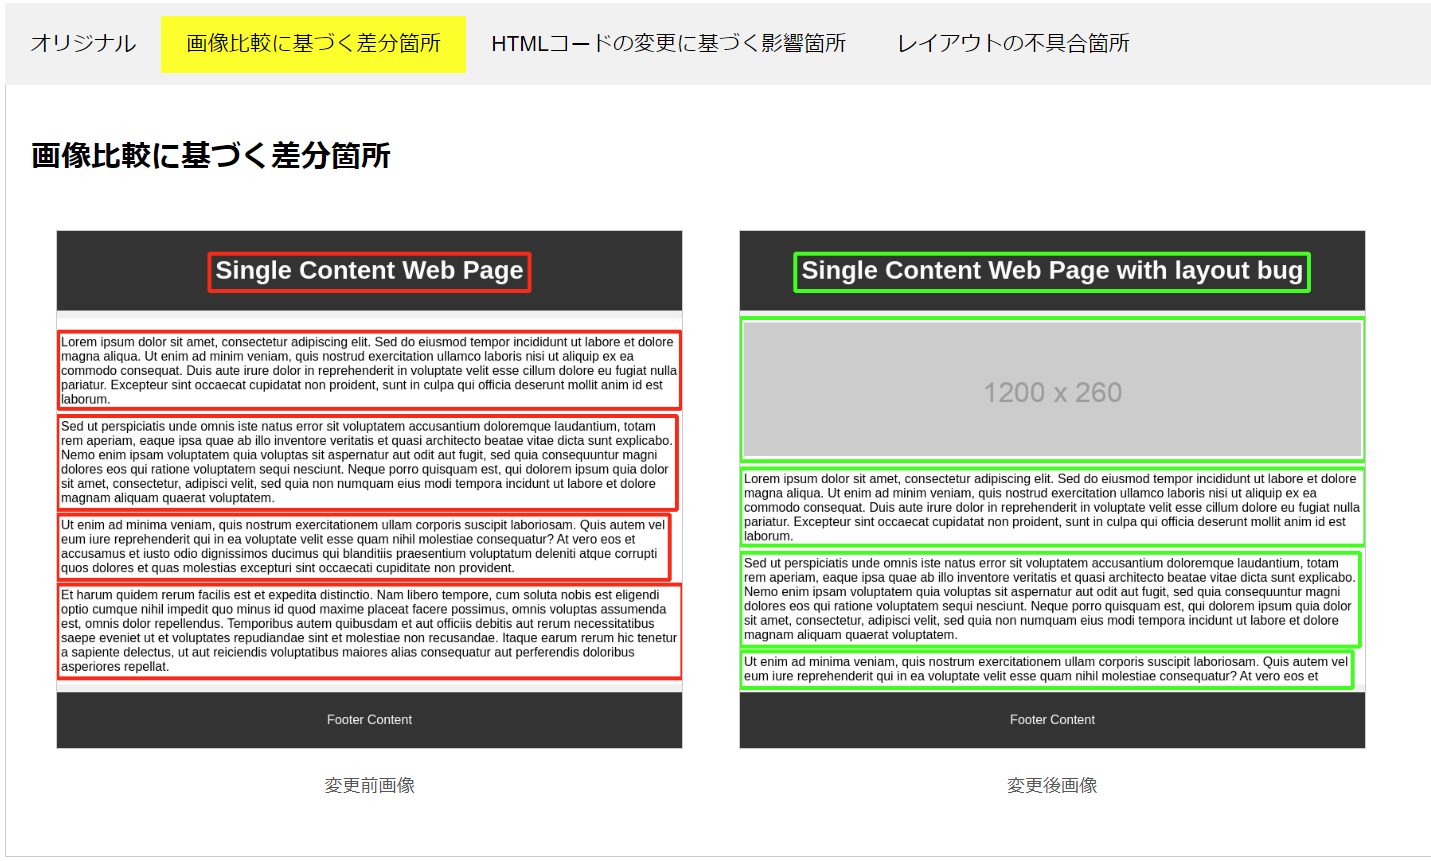
\includegraphics[width=1.0\columnwidth]{image/3_images_tab2.png}
        \caption{画像比較に基づく差分箇所表示タブを押した際の\toolName の画面例}
        \label{fig: Appearance_images_tab}
    \end{center}
\end{figure}

\subsection{HTMLコードの変更に基づく影響箇所表示タブ}\label{subsec:html_tab}
HTMLの変更に基づく影響箇所表示タブを押すと、HTMLの変更に基づく影響箇所を色付きの枠で囲んで強調表示した、Webページの変更前画像と変更後画像を並べて表示する。
HTMLの変更に基づく影響箇所表示タブを押した際の画面例を、図\ref{fig: Appearance_html_tab}に示す。
変更前のWebページのHTMLでの影響箇所は変更前画像上に赤枠で囲んで強調表示し、変更後のWebページのHTMLでの影響箇所は変更後画像上に緑枠で囲んで強調表示する。
このタブでは、図\ref{fig: Appearance_images_tab}における差分箇所から、開発者が意図して変更した、または意図せず変更してしまったHTMLコードによる影響箇所のみを目視で確認できる。
% このタブでは、変更前後のWebページで開発者が意図した、または意図しないHTMLコードの変更による影響箇所を目視で確認できる。
\begin{figure}[tp]
    \begin{center}
        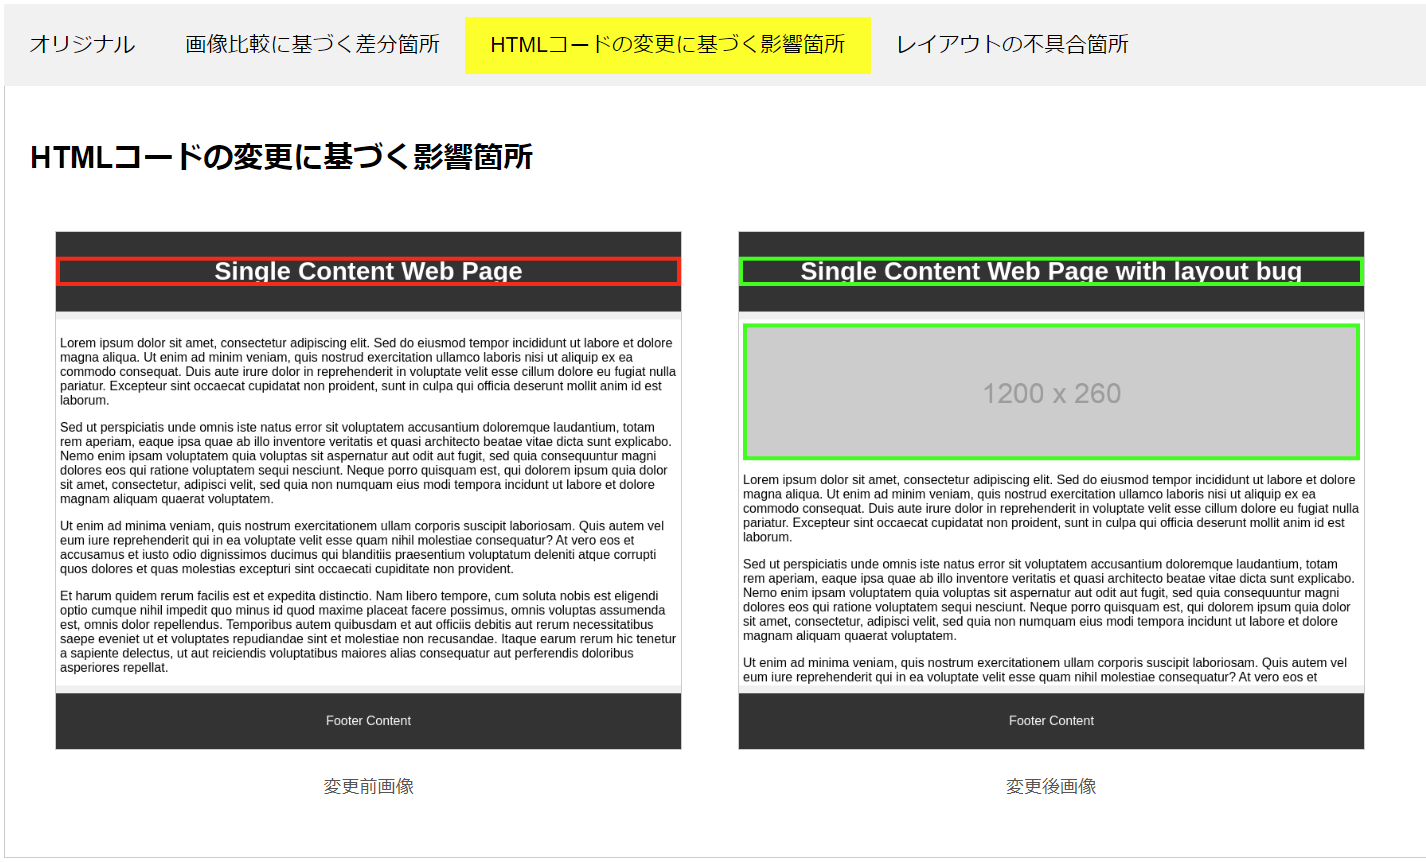
\includegraphics[width=1.0\columnwidth]{image/3_html_tab2.png}
        \caption{HTMLコードの変更に基づく影響箇所表示タブを押した際の\toolName の画面例}
        \label{fig: Appearance_html_tab}
    \end{center}
\end{figure}

\subsection{レイアウトの不具合箇所表示タブ}\label{subsec:subeffect_tab}
レイアウトの不具合箇所表示タブを押すと、差分箇所と影響箇所の比較によって検出したレイアウトの不具合箇所を色付きの枠で強調表示した、Webページの変更前画像と変更後画像を並べて表示する。
レイアウトの不具合箇所表示タブを押した際の画面例を、図\ref{fig: Appearance_subEffect_tab}に示す。
レイアウトの不具合箇所は変更前画像上に赤枠で囲んで強調表示し、レイアウトの不具合箇所は変更後画像上に緑枠で囲んで強調表示する。
このタブでは、図\ref{fig: Appearance_images_tab}における差分箇所から、レイアウトの不具合箇所のみを目視で確認できる。
\begin{figure}[tp]
    \begin{center}
        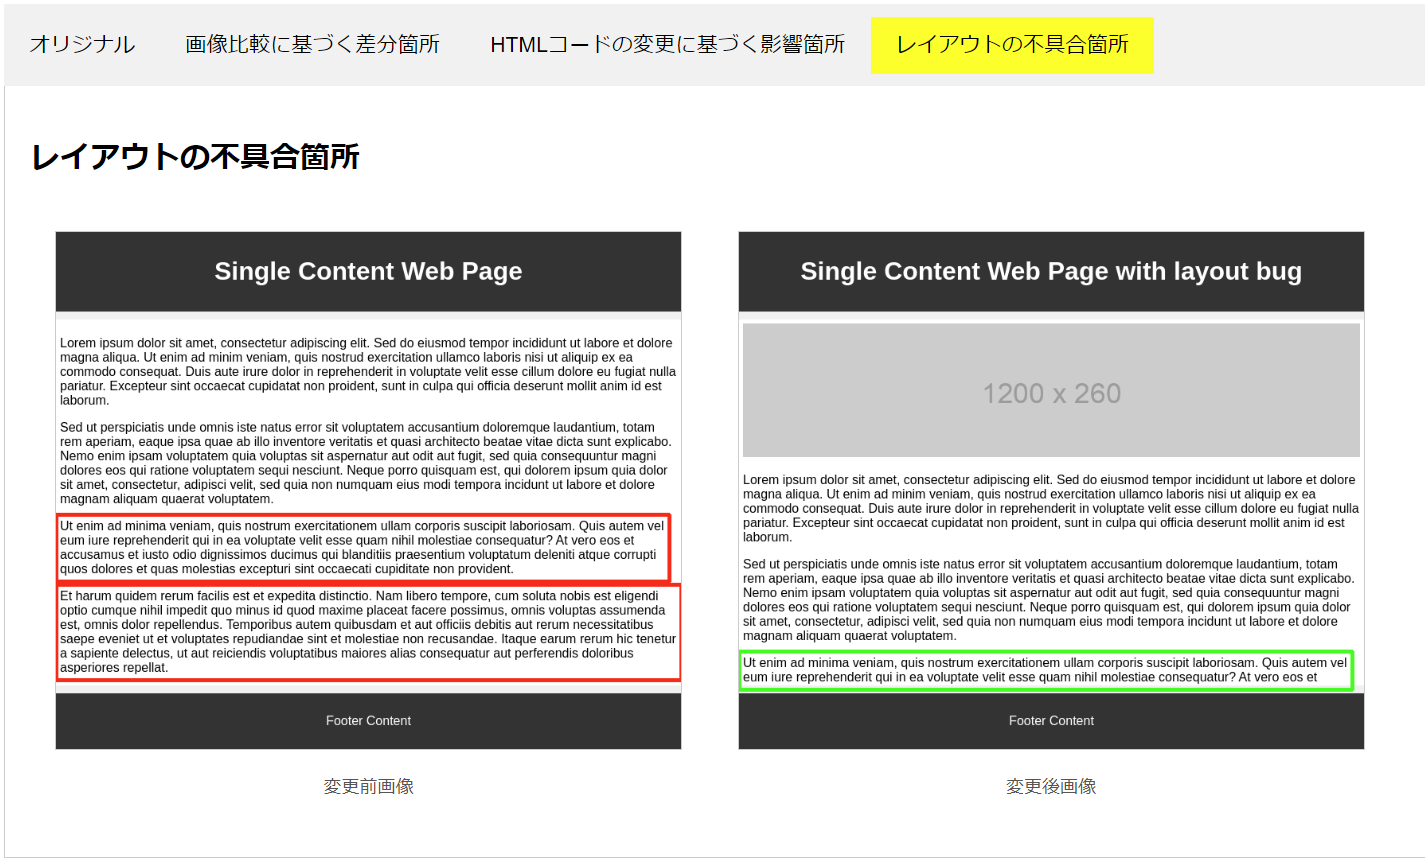
\includegraphics[width=1.0\columnwidth]{image/3_subEffect_tab2.png}
        \caption{レイアウトの不具合箇所表示タブを押した際の\toolName の画面例}
        \label{fig: Appearance_subEffect_tab}
    \end{center}
\end{figure}
